\section{Asynchronous Subsystems}
The nature of Order's requires a vary particular type of asynchronous handling.  Lucky for us we were able to find a ruby gem that makes this messy process quite elegant.  Resque allows one to queue up tasks and execute them in "first in first out"(FIFO) order by dequeueing the next enabled task in-line and performing it.  For our application we need to be able to wait before processing certain orders based on their dependencies and characteristics.  Rather then have a different data-type and handler for every type of order, we took the approach to consolidate all order types into a single order data-type that has a field that specifies the transactionType.  The orderHandler can be considered more of a wrapper function as it checks the transactionType of the order it is to perform and send it off to be handled uniquely based on the checked value.  While market orders, are executed almost immediately after being placed, stop and limit orders may not be executed for quite some time.  Whenever a task needs to be performed asynchronously, the task is entered into a designated portion of a Redis database, configured as a queue. Background "workers" (processes) perform tasks as they arrive. There are specifically two dedicated processes named Worker1 and Worker2, dedicated to order processing and UserSummary sending respectfully.  Worker two runs every 24 hours and is responsible for populating a list of one UserSummary task for each user. In order for the UserSummaryController to obtain all necessary information on user and league performance information.  The Performance Summarization objects are invoked to handle the retrieval of those specific stats, with the retrieval being handled by the DatabaseInterface object.


\subsection{Asynchronous Subsystem Diagram}
\begin{figure}[b]
\centering
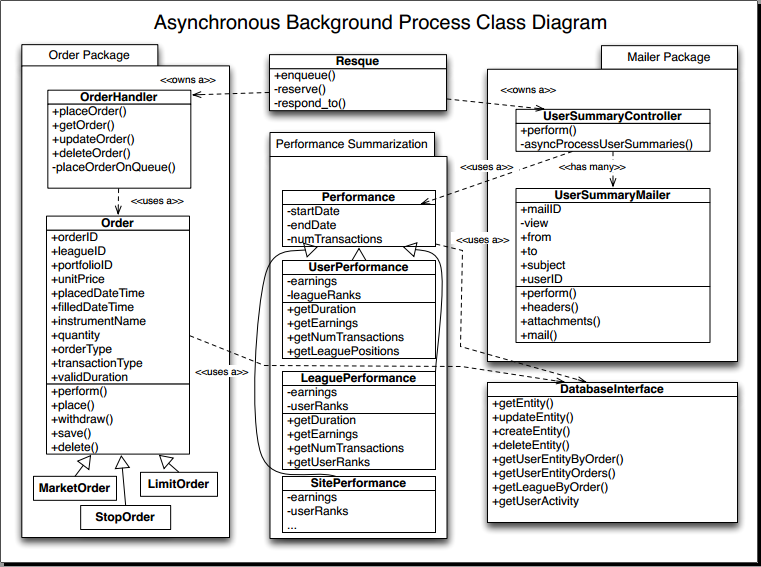
\includegraphics[width=5in]{./Diagrams/ClassDiagrams/cd2.png}
\caption{ Asynchronous Class Diagrams.}
\end{figure}


\begin{table}
\subsection{Attribute Table}
\begin{tabular}{|p{1.5in}|p{1.5in}|p{3in}|}
\hline
Concept & Attribute & Meaning\\
\hline
Task Queue & resque & resque is a ruby gem that queue's Order Handling jobs and processes them first in first out.\\
\hline
Order Handler & orderHandler & function responsible for processing orders.\\
\hline
Order & order & data type that contains order details to be processed by the orderHandler.\\
\hline
Mail Controller & UserSummaryController & handles queueing userSummaryMailer tasks and then executing them.\\
\hline
Mail Sender & UserSummaryMailer & handles the generation and sending of a single User Summary.\\
\hline
User Performance Retriever & Performance & retreives a user's performance for the User Summary.\\
\hline
League Performance Retriever & LeaguePerformance & retreives a leagues performance for the User Summary.\\
\hline
\end{tabular}
\caption{ Attribute Table.}
\end{table}
\subsection{Object Constraint Language}
To separate topics in this section, we will talk about each grouping of classes one at a time. 
\subsubsection{Order Package}
The first section of the ``Order Package'' stub is a class that deals with handling orders. The constraints for this class are the usual -- the function will work as long as they are given a correct order. That means that it has to be from a league that is in the boundary of it's date, if the order is a buy it must be under the constraint of how much money the user has and if it is a sell they must already own that much stock.\\
As of the actual order class, most of the variables in the class are but integers. The constraint on these integers is that all of them are positive, and league\_id and portfolio\_id must already exist. Also, once both variables are filled, placedDateTime must be before filledDateTime.
\subsubsection{Resque}
Resque is the simplest class in the asynchronous system as its only constraint is that it must have a valid order passed in.
\subsubsection{Performance Summarization}
The performance class has constraints on the variables startDate and endDate. These two variables only have the constraint that startDate must be earlier than endDate. It also has the constraint that the numTransactions variable must be a non-negative integer.
The rest of the variables related to Performance Summarization are integers that must also be non-negative.
\subsubsection{Mailer Package}
The mailer package class is a simple class that will succeed as long as the orders constraints went well. All of the variables in UserSummaryMailer are simple to check if they are correct, they are all strings that should not be NULL or they are integers that should represent an ID so they must be non-negative.
\subsubsection{Database Interface}
Every function in this class can do a simple check to see if the object that was passed in exists. All of the functions deal with operations on an object so checking for existance is all they will need as constraints.
